\documentclass{article} 
\usepackage{iclr2025_conference,times}


\input{math_commands.tex}

\usepackage{graphicx}
\usepackage[hypertexnames=false]{hyperref}
\usepackage{url}
\usepackage{float}


\title{Graph Neural Networks for System Call Graph-based Intrusion Detection}


\author{Raphaël Faure \& Tristan Beruard \& Sacha Dupuydauby \\
CentraleSupélec \\
\texttt{\{raphael.faure2, tristan.beruard, sacha.dupuydauby\}@student-cs.fr} \\
}

\newcommand{\fix}{\marginpar{FIX}}
\newcommand{\new}{\marginpar{NEW}}

\iclrfinalcopy 
\begin{document}


\maketitle


\begin{abstract}

Host-based intrusion detection aims to detect malicious executions from low-level traces of process activity. System calls are a natural signal for this objective because they directly expose how a program interacts with the operating system. In this report, we study two complementary questions that match the course objectives: how the choice of representation changes the learning problem, and how this choice affects robustness across tasks. We therefore compare graph-based and sequence-based models on ADFA-LD \cite{adfa} and two LID-DS scenarios \cite{lid_ds}. Our graph pipeline converts each trace into a directed weighted syscall graph and evaluates both a classical PageRank-based anomaly detector and several graph neural networks, namely GCN \cite{gcn}, GraphSAGE \cite{graphsage}, GAT \cite{gat}, and a weighted GCN variant denoted WGCN+. We also benchmark sequence-only baselines to situate the graph approach with respect to the historical syscall-sequence literature \cite{unm_syscalls}. The experiments show that graph representations are informative, but their advantage depends on the regime: GAT is strongest on ADFA-LD, whereas the PageRank and TF-IDF baselines are extremely competitive on the bruteforce LID-DS scenario. A transfer experiment across LID-DS attack families further shows that all methods degrade substantially out of distribution, with PageRank and WGCN+ remaining the most stable.
 

\end{abstract}

\section{Introduction/Motivation}

Host-based intrusion detection remains difficult because malicious activity often appears as a subtle deformation of otherwise legitimate execution traces. System call logs are attractive in this setting because they are available at the operating-system boundary and provide a detailed view of process behavior. Early work therefore modeled them directly as short sequences or sequence windows \cite{unm_syscalls,alt_syscall_models}. More recent graph-based work argues that the transition structure itself is discriminative and should be modeled explicitly \cite{syscall_graphs}. However, it remains unclear when a graph representation is actually more useful than a direct sequential one for host-based intrusion detection.

Our starting point is that a syscall trace is not only a sequence, but also a transition system. If two syscalls interact repeatedly, if a subset of calls becomes a hub, or if unusual loops emerge, this structure is naturally visible in a graph representation. This motivates our main research questions: does a syscall-graph representation improve host-based intrusion detection, which graph models are the most relevant for these data, and how stable are these conclusions across datasets and attack scenarios?

The practical motivation is straightforward. Better host-based intrusion detection can support endpoint protection, anomaly triage, incident response, and post-compromise forensics. From a machine learning perspective, the project also provides a useful case study for comparing interpretable graph scoring methods with learned graph representations on a real cybersecurity task.



\section{Problem Definition}

Let a syscall trace be a sequence $s=(x_1,\dots,x_T)$, where each token $x_t$ is either an integer syscall identifier, as in ADFA-LD, or a syscall name extracted from a raw trace, as in LID-DS. From each sequence we build a directed weighted graph $G=(V,E,w)$ where each node in $V$ is a unique syscall and each edge $(u,v)\in E$ records the number of times syscall $u$ is immediately followed by syscall $v$ in the trace.

The supervised task is binary graph classification. Given a trace graph $G_i$ and its label $y_i\in\{0,1\}$, with $0$ denoting normal behavior and $1$ an attack trace, we seek a predictor $f(G_i)\rightarrow \hat{y}_i$. Because the datasets are imbalanced and scenario-dependent, we evaluate the predictor with accuracy, precision, recall, F1 score, and ROC-AUC rather than relying on accuracy alone.

We also consider an anomaly-detection baseline based on PageRank. In that setting, the training procedure builds a normal library from benign traces only and the decision is taken from an anomaly score computed on sliding windows. Concretely, for a fixed window length $m$, a trace $s=(x_1,\dots,x_T)$ is decomposed into overlapping subsequences $w_t=(x_t,\dots,x_{t+m-1})$ for $t=1,\dots,T-m+1$. Each window is compared with a library of normal patterns, and the final anomaly score is the fraction of windows whose distance to that library exceeds a chosen threshold. The problem then becomes threshold-based anomaly scoring instead of direct discriminative classification.

\section{Related Work} 
System call based intrusion detection has historically been studied through sequence models and symbolic matching rules because the data naturally arrives as an ordered stream. The classical UNM line of work \cite{unm_syscalls,alt_syscall_models} showed that short syscall windows already provide a strong anomaly-detection signal, which remains an important baseline for any newer approach. Graph-based approaches instead argue that transition structure itself is discriminative and should therefore be modeled explicitly. The system-call graph formulation of Grimmer et al. \cite{syscall_graphs} is particularly relevant here because it motivates representing a trace by its directed transition graph rather than by sequence statistics only.

On the representation-learning side, graph neural networks provide a natural way to combine local transition structure with node-level attributes. GCN \cite{gcn} is a standard baseline based on neighborhood aggregation, while GraphSAGE \cite{graphsage} and GAT \cite{gat} extend this idea respectively through flexible aggregation and attention over neighbors. Although these families are widely used in graph learning, they remain comparatively underexplored for host-based intrusion detection on syscall graphs.

Our classical baseline is related to the PageRank anomaly scoring strategy of \cite{pagerank_ids}. The original idea is to derive transition suspiciousness from a PageRank-weighted normal graph and then measure the distance between observed windows and a library of normal patterns. Our implementation keeps this core mechanism but adapts it to a multi-trace training pipeline and to reproducible Hydra-based experiments.







\section{Methodology} 

\paragraph{Datasets and preprocessing.}
We use two host-based intrusion detection datasets. ADFA-LD \cite{adfa} provides integer-encoded syscall traces with separate normal and attack folders. LID-DS \cite{lid_ds} provides richer per-sample archives containing raw \texttt{.sc} traces and metadata. For LID-DS, our final study focuses on the scenarios \texttt{Bruteforce\_CWE-307} and \texttt{CVE-2014-0160}. Within each retained scenario, we use a standard stratified train/validation/test split.

\paragraph{Graph construction and node features.}
Each trace is converted into a directed weighted graph. For ADFA-LD, node features include relative frequency, in/out degree, weighted degree, PageRank, and self-loop indicators. For LID-DS, we enrich the representation with process diversity, return-value statistics, and temporal gap statistics recovered from the raw traces. More precisely, the additional LID-DS features summarize how many distinct processes emit a syscall, how often it returns errors, the empirical moments of its return values, and the typical time gaps before and after this syscall. Each graph is then turned into a PyTorch Geometric object with both numeric node features and a learned embedding for the syscall identity. Unless otherwise stated, the default GNN configuration uses the full node-feature profile together with weighted edges.

\paragraph{Feature variation.}
The graph representation itself is a design choice, so we explicitly study how the selected node and edge features affect performance. On the node side, we consider progressively richer profiles. The simplest setting uses only the learned syscall identity embedding, which tests whether structural propagation alone is sufficient. A second family of profiles uses structural descriptors such as degree, weighted degree, PageRank, and self-loop indicators. On LID-DS, a richer profile additionally includes behavioral statistics extracted from the raw traces: error rates indicate whether a syscall often fails, return-value moments summarize the dispersion of its outputs, process diversity measures how many distinct processes or execution contexts emit it, and temporal gaps capture whether it tends to appear in bursts or after long pauses. On the edge side, we compare two regimes: binary edges, where an observed transition is represented only by its existence, and weighted edges, where the multiplicity of a transition is preserved. This ablation is important because syscall graphs can encode both \emph{which} transitions exist and \emph{how often} they occur, and these two signals need not contribute equally across scenarios.

\paragraph{PageRank baseline.}
The PageRank detector follows a classical anomaly-detection logic. We build a normal transition graph, compute PageRank scores, derive a suspiciousness map $k(u,v)$ from the weighted outgoing contribution of each transition, slide a fixed-size window over the observed sequence, and score each observed window by its minimum weighted distance to a normal pattern. The final anomaly score is the proportion of windows whose distance exceeds a threshold.

The production implementation makes three engineering adaptations. First, the pattern library is built from all normal training traces instead of a single file. Second, we use pattern subsampling, caching, and prefix-based candidate filtering to keep evaluation tractable on larger datasets. Third, the distance and anomaly thresholds are selected on the validation split rather than fixed manually. The mathematical core of the method is therefore preserved while the training protocol is generalized to our datasets.

\paragraph{Sequence-only baselines.}
To complement the graph-based view, we also evaluate models that operate directly on the syscall sequence without explicitly building a graph. These baselines are important because they connect our study to the historical syscall-sequence literature initiated by the UNM work \cite{unm_syscalls,alt_syscall_models}. The first baseline is a TF-IDF representation of syscall $n$-grams followed by logistic regression. If $\phi(s_i)$ denotes the sparse TF-IDF vector extracted from a trace $s_i$, the classifier predicts
\[
p(y_i=1 \mid s_i) = \sigma(w^\top \phi(s_i) + b).
\]
This baseline captures local order statistics and repeated motifs very efficiently, but it does not explicitly model long-range transition structure beyond the selected $n$-gram window.

The second baseline is a bidirectional GRU sequence encoder. Given embedded tokens $e(x_t)$, the recurrent state is updated as
\[
h_t = \mathrm{GRU}(e(x_t), h_{t-1}),
\]
and the final representation is passed to a small MLP classifier. This approach preserves sequential order more faithfully than TF-IDF, but in practice it requires truncating long traces to keep training tractable. In our implementation, this makes the GRU more sensitive to sequence length and to where discriminative events occur inside the trace.

\paragraph{GNN models.}
We compare four graph neural architectures. In all cases, each node $v$ starts from an initial representation
\[
h_v^{(0)} = [\,e(\mathrm{syscall}_v)\, \Vert \, x_v\,],
\]
where $e(\mathrm{syscall}_v)$ is a learned embedding of the syscall identity and $x_v$ is the handcrafted numeric feature vector. Let $A$ denote the weighted adjacency matrix, with $A_{uv}$ equal to the number of observed transitions from syscall $u$ to syscall $v$, and let $\mathcal{N}(v)$ be the neighborhood of $v$.

The first baseline is the Graph Convolutional Network (GCN) \cite{gcn}. In matrix form, a layer can be written as
\[
H^{(\ell+1)} = \sigma\!\left(\hat{D}^{-1/2}\hat{A}\hat{D}^{-1/2} H^{(\ell)} W^{(\ell)}\right),
\]
where $\hat{A}=A+I$ adds self-loops, $\hat{D}$ is the associated degree matrix, $W^{(\ell)}$ is a learnable weight matrix, and $\sigma$ is a pointwise non-linearity. Intuitively, GCN smooths node representations over the local transition structure. This is relevant for syscall graphs because normal executions often induce repeated and locally coherent transition motifs. Its limitation is that all neighbors are mixed through the same normalized operator, which can blur rare but important malicious transitions.

The second baseline is GraphSAGE \cite{graphsage}, which separates the representation of a node from the aggregate of its neighbors:
\[
m_v^{(\ell)} = \mathrm{MEAN}\{h_u^{(\ell)} : u \in \mathcal{N}(v)\}, \qquad
h_v^{(\ell+1)} = \sigma\!\left(W_{\mathrm{self}}^{(\ell)} h_v^{(\ell)} + W_{\mathrm{neigh}}^{(\ell)} m_v^{(\ell)}\right).
\]
This formulation is useful when one expects the node's own state and its neighborhood context to play different roles. Compared with GCN, GraphSAGE can also be slightly more robust to over-smoothing, that is, to the regime where repeated neighborhood averaging makes the embeddings of different nodes nearly indistinguishable after several layers. For syscall graphs, this matters because rare syscall roles can disappear if every node becomes too similar to its neighbors.

The third baseline is the Graph Attention Network (GAT) \cite{gat}. Instead of averaging neighbors uniformly after normalization, GAT learns attention coefficients:
\[
\alpha_{vu}^{(\ell)} = \mathrm{softmax}_{u \in \mathcal{N}(v)}\left(
\mathrm{LeakyReLU}\!\left(a^{\top}[W h_v^{(\ell)} \Vert W h_u^{(\ell)} \Vert \phi(e_{vu})]\right)
\right),
\]
\[
h_v^{(\ell+1)} = \sigma\!\left(\sum_{u \in \mathcal{N}(v)} \alpha_{vu}^{(\ell)} W h_u^{(\ell)}\right),
\]
where $\phi(e_{vu})$ denotes the edge attribute derived from the transition weight. This mechanism is particularly appealing for intrusion detection because not all syscall transitions are equally informative. A few rare edges can carry a large fraction of the malicious signal, and attention allows the model to focus more strongly on these transitions. This is one reason why GAT is a plausible candidate on ADFA-LD, where attack traces often differ through specific localized changes in transition importance rather than through a uniform deformation of the whole graph.

Finally, our main architecture is denoted \textbf{WGCN+}. It keeps the weighted GCN propagation rule above, but adds two modifications tailored to the current data regime. First, after each message-passing layer we apply layer normalization, which stabilizes hidden representations when graph sizes and degrees vary across samples. Second, instead of a single global pooling operator, we concatenate mean pooling and max pooling:
\[
g_G = \left[\mathrm{MeanPool}\!\left(H^{(L)}\right) \Vert \mathrm{MaxPool}\!\left(H^{(L)}\right)\right].
\]
Mean pooling summarizes the average execution profile of the trace, while max pooling preserves the strongest activated motifs. This combination is well suited to syscall graphs because an attack can manifest both as a global redistribution of transition statistics and as a small set of highly abnormal local patterns. In practice, we expect GCN-like models to be favored when the signal is distributed across many transitions, and GAT to be favored when a small number of edges carry disproportionate discriminative information.

\paragraph{Training protocol.}
All GNN models are trained with Adam and selected using validation F1. The best validation checkpoint is then evaluated on the held-out test split. The report figures and tables are exported automatically from the training pipeline so that the manuscript remains synchronized with the actual experimental artifacts.

\paragraph{Learning paradigms.}
Beyond standard supervised classification, we evaluate one additional learning setting. In the supervised setting, the encoder and classifier are trained end-to-end with the binary cross-entropy classification objective implemented through the usual softmax cross-entropy loss
\[
\mathcal{L}_{\mathrm{sup}} = - \sum_{i=1}^{N} \log p_\theta(y_i \mid G_i).
\]
This is the most direct setting when graph labels are available for all training samples.

In the anomaly-detection setting, the encoder is trained mainly on normal graphs. Let $g_i$ denote the graph embedding of a normal sample and let $c$ be the center of the normal embedding cloud. We minimize a one-class objective inspired by Deep SVDD \cite{deep_svdd}, where the model learns a compact hypersphere containing normal samples:
\[
\mathcal{L}_{\mathrm{ano}} = \frac{1}{N_{\mathrm{normal}}} \sum_{i=1}^{N_{\mathrm{normal}}} \|g_i - c\|_2^2.
\]
At inference time, the anomaly score is the squared distance $\|g-c\|_2^2$, and the decision threshold is selected on the validation split. This setting is relevant for intrusion detection because in realistic deployments normal traces are often abundant while attack labels are scarce or incomplete.

\paragraph{Cross-scenario protocol.}
To study out-of-distribution generalization on LID-DS, we define a transfer setting from \texttt{Bruteforce\_CWE-307} to \texttt{CVE-2014-0160}. We train and tune the model on the source scenario only, then evaluate it unchanged on the target scenario. This protocol deliberately introduces a scenario shift between source and target attacks while keeping model selection entirely on the source scenario.
\IfFileExists{generated_graph_inspection.tex}{% Auto-generated graph inspection block.
\subsection{Graph Inspection}
The generated syscall graphs remain in a small-to-medium regime while staying fairly dense: ADFA-LD contains 5951 graphs with 19.9 nodes and 57.3 edges on average (directed density 0.245); LID-DS (Bruteforce\_CWE-307) contains 907 graphs with 29.5 nodes and 240.5 edges on average (directed density 0.283); LID-DS (CVE-2014-0160) contains 878 graphs with 29.8 nodes and 113.8 edges on average (directed density 0.132). This profile makes local message-passing models appropriate because each node interacts with a limited but informative neighborhood, so a few propagation steps can aggregate most of the useful local transition context without requiring very deep architectures. We therefore compare a plain GCN baseline, GraphSAGE for more robust neighborhood aggregation, GAT to test whether attention over heterogeneous syscall transitions improves discrimination, and our WGCN+ variant that combines weighted GCN propagation, learned syscall embeddings, structural node features, layer normalization, and hybrid graph pooling.

\begin{table}[H]
\centering
\resizebox{\linewidth}{!}{%
\begin{tabular}{lrrrrrr}
\hline
Dataset & Graphs & Attack \% & Mean $|V|$ & Mean $|E|$ & Mean density & Mean seq. len. \\
\hline
ADFA-LD & 5951 & 12.54 & 19.94 & 57.29 & 0.24 & 461.70 \\
LID-DS (Bruteforce\_CWE-307) & 907 & 15.33 & 29.47 & 240.53 & 0.28 & 8136.46 \\
LID-DS (CVE-2014-0160) & 878 & 13.67 & 29.78 & 113.81 & 0.13 & 1640.26 \\
\hline
\end{tabular}
}
\caption{Graph-level inspection of the datasets used by the training pipeline, computed on the same trace pools as the reported experiments.}
\label{tab:graph-inspection}
\end{table}

\begin{figure}[H]
\centering
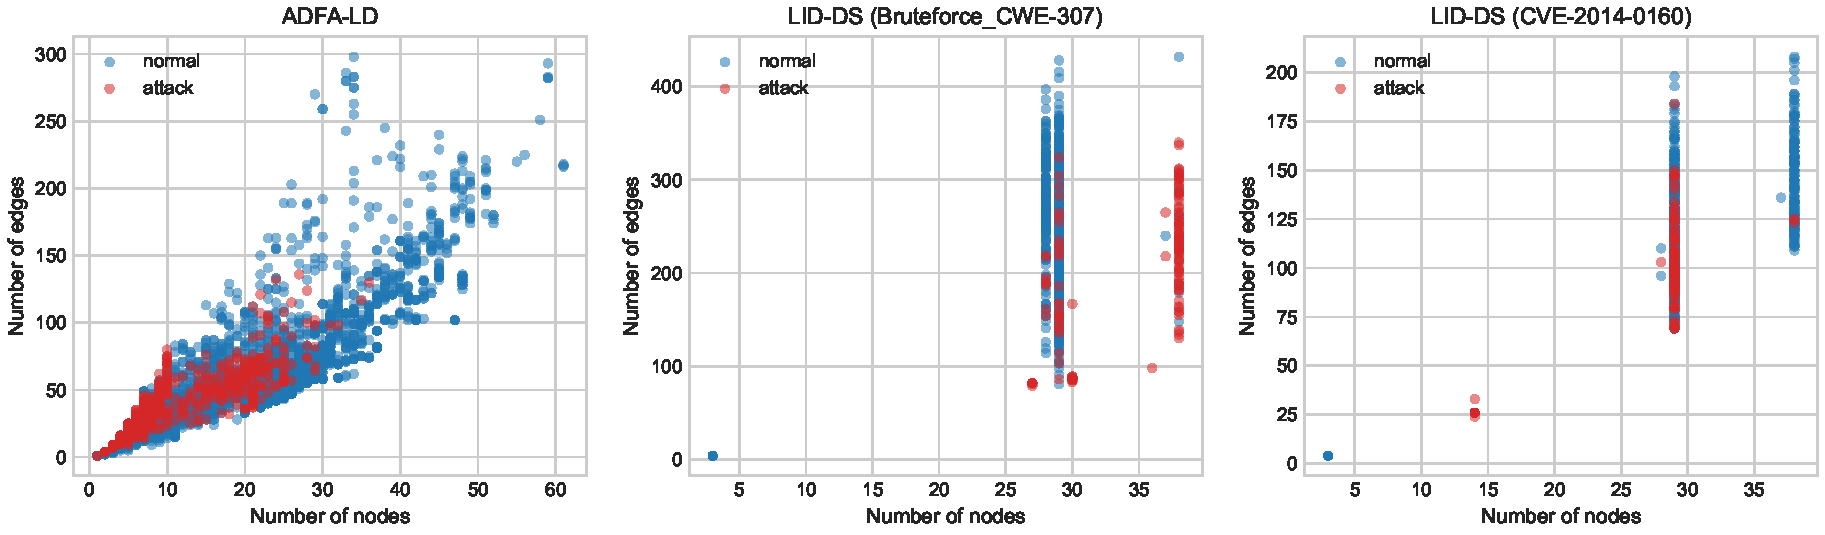
\includegraphics[width=0.72\linewidth]{figures/graph_nodes_edges_scatter.pdf}
\caption{Number of nodes versus number of edges for the generated syscall graphs, colored by class.}
\label{fig:graph-inspection}
\end{figure}
}{}

\section{Evaluation}

\paragraph{Experimental setting.}
The benchmark combines PageRank, GCN, GraphSAGE, GAT, and WGCN+ on ADFA-LD. On LID-DS, we report PageRank and WGCN+ on the two retained scenarios. In addition to this main benchmark, we run a feature ablation on \texttt{LID-DS / Bruteforce\_CWE-307}, a comparison between supervised and anomaly-detection training for WGCN+ on ADFA-LD, a comparison against sequence-only baselines, and a cross-scenario transfer experiment from \texttt{Bruteforce\_CWE-307} to \texttt{CVE-2014-0160}. The sequence baselines are TF-IDF $n$-gram logistic regression and a bidirectional GRU. The third scenario initially considered, \texttt{CWE-89-SQL-injection}, was removed from the final study because preprocessing and graph construction on this scenario exceeded the available memory budget in our environment.

\paragraph{Main observations.}
Three conclusions stand out from the benchmark reported in Table~\ref{tab:automated-results}. First, on ADFA-LD, all GNN variants clearly outperform the PageRank baseline in ROC-AUC and F1, and GAT achieves the best overall test performance. This suggests that, on ADFA-LD, heterogeneous transition importance matters and is captured well by attention. Second, on the LID-DS bruteforce scenario, both approaches are very strong, but the PageRank baseline is actually the best method in our experiments, which indicates that this scenario is dominated by highly regular local transition anomalies that can already be captured by the window-based normal-pattern library. Third, on the harder \texttt{CVE-2014-0160} scenario, PageRank remains imperfect but usable, whereas WGCN+ reaches high ROC-AUC yet collapses to zero F1 under the default classification threshold. This means the model still ranks traces reasonably well, but its final decision boundary is poorly calibrated under this scenario.

\paragraph{Feature ablation.}
The feature ablation in Table~\ref{tab:feature-ablation} confirms that representation design matters substantially on LID-DS. Using only syscall embeddings and binary edges already yields a non-trivial result ($F1=0.7843$), which shows that graph topology and syscall identity alone contain useful information. Adding structural node descriptors improves the result to $F1=0.8085$, but the main jump appears when the richer handcrafted features are reintroduced: the full node profile with binary edges reaches $F1=0.8679$. Finally, restoring weighted edges gives the best configuration with $F1=0.9231$ and $ROC$-$AUC=0.9782$. This progression is consistent with the problem structure: the bruteforce scenario is not characterized only by which transitions occur, but also by how often they are repeated and by the statistics attached to the involved syscalls.

\paragraph{Learning paradigms.}
The comparison of learning paradigms in Table~\ref{tab:learning-paradigms} follows the expected ranking under our current implementation budget. Supervised learning is the strongest setting, with $F1=0.8322$ and $ROC$-$AUC=0.9851$, because it directly optimizes the discriminative objective of interest. The anomaly-detection setting is weaker ($F1=0.4875$, $ROC$-$AUC=0.8497$), but it remains informative as a realistic deployment scenario in which one primarily models normal behavior and detects deviations by distance in embedding space.

\paragraph{Sequence-only baselines.}
The sequence baselines in Table~\ref{tab:sequence-baselines} produce a nuanced picture. On ADFA-LD, both sequence-only models are competitive: TF-IDF logistic regression reaches $F1=0.7692$ and the GRU reaches $F1=0.7708$, both with ROC-AUC close to $0.98$. This means that on ADFA-LD a large fraction of the signal is already present in local sequential motifs. However, both remain below the best graph models, especially GAT, which suggests that the graph abstraction still captures useful transition structure beyond raw local $n$-grams. On \texttt{LID-DS / Bruteforce\_CWE-307}, the TF-IDF baseline is extremely strong ($F1=0.9630$, $ROC$-$AUC=1.0000$), on par with the strongest graph-based results, whereas the GRU performs poorly ($F1=0.1765$). A plausible explanation is that the bruteforce traces are long and repetitive: a sparse bag of local motifs still captures these repetitions well, while the truncated recurrent encoder struggles with long-range dependencies and with discriminative events that may appear far from the retained sequence prefix.

\paragraph{Cross-scenario generalization.}
The transfer experiment in Table~\ref{tab:cross-scenario-generalization} reveals a clear loss of generalization across attack scenarios. WGCN+ drops to $F1=0.3217$ and $ROC$-$AUC=0.7058$ on the target scenario, even though it performs very well on the source validation split. TF-IDF logistic regression degrades further to $F1=0.2012$ and ROC-AUC $0.5783$, while the GRU almost collapses completely ($F1=0.0382$). Interestingly, the PageRank detector remains competitive in this transfer setting ($F1=0.3519$, $ROC$-$AUC=0.7045$), likely because its anomaly score is anchored in deviations from normal local transition patterns rather than in a fully discriminative source-task boundary. Overall, these results suggest that the representation learned from one attack family does not transfer cleanly to another on LID-DS, and that scenario shift is a major challenge for host-based intrusion detection.

\paragraph{Interpretation and limitations.}
The graph inspection in Table~\ref{tab:graph-inspection} and Figure~\ref{fig:graph-inspection}, the benchmark in Table~\ref{tab:automated-results}, and the ablations in Table~\ref{tab:feature-ablation} together suggest that there is no single winner across all operating conditions, but that the best method can be understood from the data regime. Dense and repetitive scenarios such as bruteforce attacks are particularly favorable to local pattern methods: PageRank and TF-IDF both perform extremely well there because they focus on repeated transition motifs. The feature ablation further shows that WGCN+ benefits from preserving both richer node descriptors and transition multiplicities, which is coherent with the fact that these graphs encode repeated process behavior. By contrast, ADFA-LD benefits more from learned graph representations, especially attention-based ones, although the strong ADFA-LD sequence baselines also show that sequential information alone already carries a large portion of the signal. Finally, the transfer experiment highlights a major limitation of all discriminative approaches considered here: training on one attack scenario does not ensure robust generalization to another. The current study nevertheless remains limited by CPU-only training, by the exclusion of the SQL injection scenario, and by the absence of a more systematic threshold-calibration stage for GNN outputs.
\IfFileExists{generated_results.tex}{% Auto-generated by intrusion_detection. Do not edit manually.
\newcommand{\ResultAdfaLdPagerankAccuracy}{0.8128}
\newcommand{\ResultAdfaLdPagerankFOne}{0.4652}
\newcommand{\ResultAdfaLdPagerankPrecision}{0.3619}
\newcommand{\ResultAdfaLdPagerankRecall}{0.6510}
\newcommand{\ResultAdfaLdPagerankRocAuc}{0.8092}
\newcommand{\ResultAdfaLdPagerankSupport}{1191}
\newcommand{\ResultAdfaLdWgcnPlusAccuracy}{0.9244}
\newcommand{\ResultAdfaLdWgcnPlusFOne}{0.7289}
\newcommand{\ResultAdfaLdWgcnPlusPrecision}{0.6612}
\newcommand{\ResultAdfaLdWgcnPlusRecall}{0.8121}
\newcommand{\ResultAdfaLdWgcnPlusRocAuc}{0.9636}
\newcommand{\ResultAdfaLdWgcnPlusSupport}{1191}
\newcommand{\ResultAdfaLdGcnAccuracy}{0.9362}
\newcommand{\ResultAdfaLdGcnFOne}{0.7164}
\newcommand{\ResultAdfaLdGcnPrecision}{0.8067}
\newcommand{\ResultAdfaLdGcnRecall}{0.6443}
\newcommand{\ResultAdfaLdGcnRocAuc}{0.9567}
\newcommand{\ResultAdfaLdGcnSupport}{1191}
\newcommand{\ResultAdfaLdGraphsageAccuracy}{0.9337}
\newcommand{\ResultAdfaLdGraphsageFOne}{0.7208}
\newcommand{\ResultAdfaLdGraphsagePrecision}{0.7612}
\newcommand{\ResultAdfaLdGraphsageRecall}{0.6846}
\newcommand{\ResultAdfaLdGraphsageRocAuc}{0.9617}
\newcommand{\ResultAdfaLdGraphsageSupport}{1191}
\newcommand{\ResultAdfaLdGatAccuracy}{0.9488}
\newcommand{\ResultAdfaLdGatFOne}{0.7987}
\newcommand{\ResultAdfaLdGatPrecision}{0.7857}
\newcommand{\ResultAdfaLdGatRecall}{0.8121}
\newcommand{\ResultAdfaLdGatRocAuc}{0.9790}
\newcommand{\ResultAdfaLdGatSupport}{1191}
\newcommand{\ResultLidBruteforcePagerankAccuracy}{0.9890}
\newcommand{\ResultLidBruteforcePagerankFOne}{0.9630}
\newcommand{\ResultLidBruteforcePagerankPrecision}{1.0000}
\newcommand{\ResultLidBruteforcePagerankRecall}{0.9286}
\newcommand{\ResultLidBruteforcePagerankRocAuc}{1.0000}
\newcommand{\ResultLidBruteforcePagerankSupport}{182}
\newcommand{\ResultLidBruteforceWgcnPlusAccuracy}{0.9560}
\newcommand{\ResultLidBruteforceWgcnPlusFOne}{0.8462}
\newcommand{\ResultLidBruteforceWgcnPlusPrecision}{0.9167}
\newcommand{\ResultLidBruteforceWgcnPlusRecall}{0.7857}
\newcommand{\ResultLidBruteforceWgcnPlusRocAuc}{0.9666}
\newcommand{\ResultLidBruteforceWgcnPlusSupport}{182}
\newcommand{\ResultLidCvePagerankAccuracy}{0.8864}
\newcommand{\ResultLidCvePagerankFOne}{0.3750}
\newcommand{\ResultLidCvePagerankPrecision}{0.7500}
\newcommand{\ResultLidCvePagerankRecall}{0.2500}
\newcommand{\ResultLidCvePagerankRocAuc}{0.7818}
\newcommand{\ResultLidCvePagerankSupport}{176}
\newcommand{\ResultLidCveWgcnPlusAccuracy}{0.8636}
\newcommand{\ResultLidCveWgcnPlusFOne}{0.0000}
\newcommand{\ResultLidCveWgcnPlusPrecision}{0.0000}
\newcommand{\ResultLidCveWgcnPlusRecall}{0.0000}
\newcommand{\ResultLidCveWgcnPlusRocAuc}{0.9380}
\newcommand{\ResultLidCveWgcnPlusSupport}{176}

\subsection{Automated Results}
\begin{table}[t]
\centering
\resizebox{\linewidth}{!}{%
\begin{tabular}{lllrrrrr}
\hline
Dataset & Scenario & Model & Acc. & F1 & Prec. & Rec. & ROC-AUC \\
\hline
adfa\_ld & all & pagerank & 0.8128 & 0.4652 & 0.3619 & 0.6510 & 0.8092 \\
adfa\_ld & all & gnn:wgcn\_plus & 0.9244 & 0.7289 & 0.6612 & 0.8121 & 0.9636 \\
adfa\_ld & all & gnn:gcn & 0.9362 & 0.7164 & 0.8067 & 0.6443 & 0.9567 \\
adfa\_ld & all & gnn:graphsage & 0.9337 & 0.7208 & 0.7612 & 0.6846 & 0.9617 \\
adfa\_ld & all & gnn:gat & 0.9488 & 0.7987 & 0.7857 & 0.8121 & 0.9790 \\
lid\_ds & Bruteforce\_CWE-307 & pagerank & 0.9890 & 0.9630 & 1.0000 & 0.9286 & 1.0000 \\
lid\_ds & Bruteforce\_CWE-307 & gnn:wgcn\_plus & 0.9560 & 0.8462 & 0.9167 & 0.7857 & 0.9666 \\
lid\_ds & CVE-2014-0160 & pagerank & 0.8864 & 0.3750 & 0.7500 & 0.2500 & 0.7818 \\
lid\_ds & CVE-2014-0160 & gnn:wgcn\_plus & 0.8636 & 0.0000 & 0.0000 & 0.0000 & 0.9380 \\
\hline
\end{tabular}
}
\caption{Test-set metrics exported automatically from the training pipeline.}
\label{tab:automated-results}
\end{table}

\subsection{Diagnostics: adfa\_ld\_pagerank}
\begin{figure}[t]
\centering
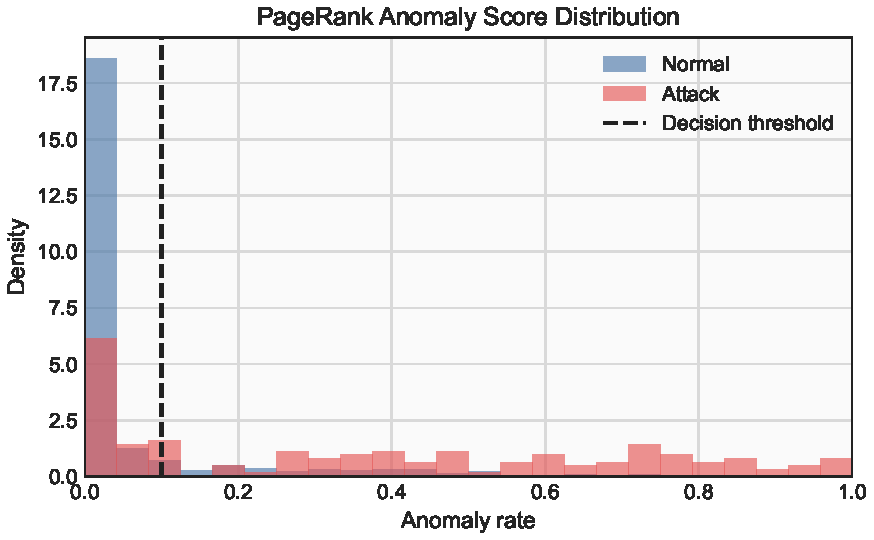
\includegraphics[width=0.7\linewidth]{figures/adfa_ld_pagerank_scores.pdf}
\caption{Diagnostic plot for \texttt{adfa\_ld\_pagerank}: distribution of test anomaly scores with the decision threshold.}
\end{figure}
\subsection{Diagnostics: adfa\_ld\_gat}
\begin{figure}[t]
\centering
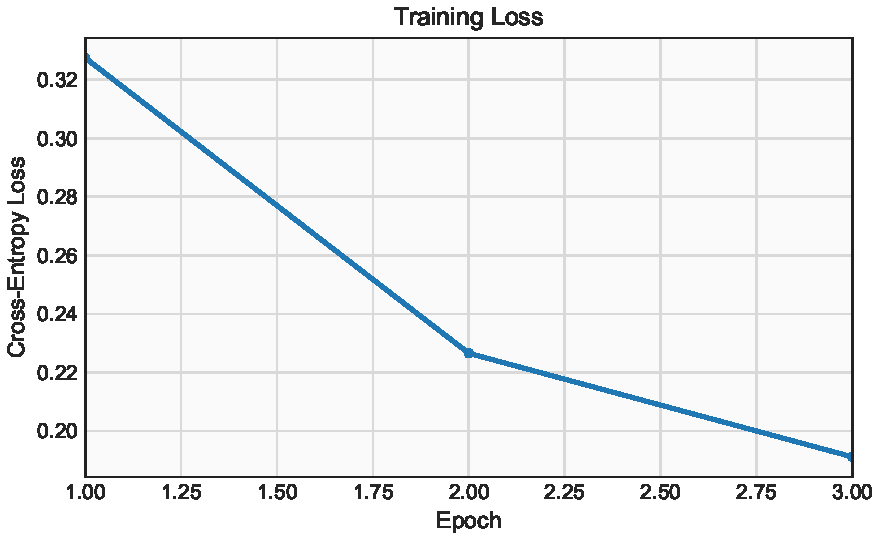
\includegraphics[width=0.48\linewidth]{figures/adfa_ld_gat_loss.pdf}
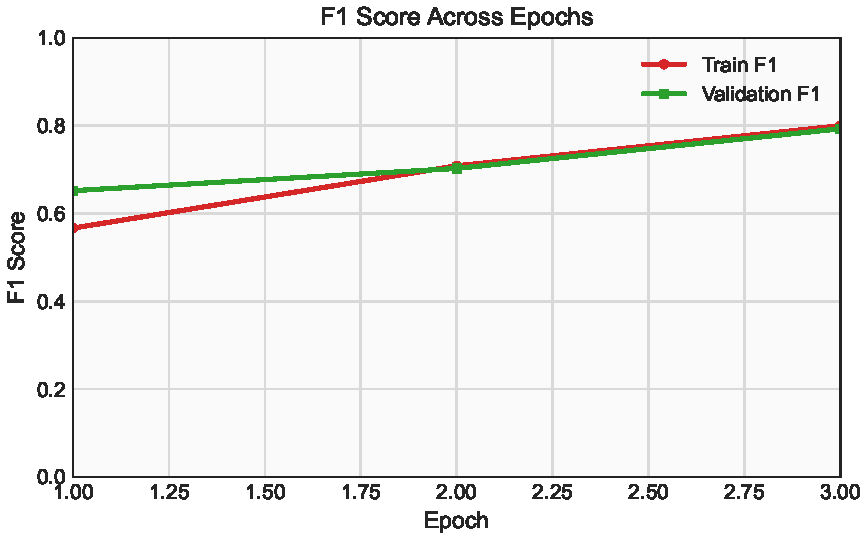
\includegraphics[width=0.48\linewidth]{figures/adfa_ld_gat_f1.pdf}
\caption{Training diagnostics for \texttt{adfa\_ld\_gat}: cross-entropy loss and F1 score as a function of epoch.}
\end{figure}
}{}



\section{Conclusions}
This project shows that syscall graphs form a useful and operational representation for host-based intrusion detection. The graph construction step preserves transition structure while enabling both classical graph scoring and graph neural message passing. In our experiments, GAT provides the strongest results on ADFA-LD, whereas the PageRank baseline remains remarkably effective on the bruteforce LID-DS scenario. The main lesson is therefore not that one model dominates everywhere, but that graph-based modeling exposes structure that different families of methods can exploit in complementary ways.

Several extensions follow naturally from this work. A first direction is to calibrate the GNN decision threshold on the validation split in the same spirit as the PageRank baseline, especially for difficult imbalanced scenarios such as \texttt{CVE-2014-0160}. A second direction is to include the SQL injection scenario once a more memory-efficient preprocessing path is available. Finally, richer dynamic or provenance-aware graph constructions could help incorporate longer-range temporal context beyond immediate syscall transitions.


\section{References}

\bibliographystyle{iclr2025_conference}
\bibliography{references}




% % - https://www.cs.unm.edu/~forrest/publications/int_decssc.pdf -> Intrusion Detection using Sequences of System Calls; simple sequence models
% - A Modern and Sophisticated Host Based Intrusion Detection Data Set LID-DS dataset
% - https://old.dbs.uni-leipzig.de/file/Intrusion-Detection-on-System-Call-Graphs.pdf -> Intrusion Detection on System Call Graphs, classification using features 
% - https://arxiv.org/pdf/2509.16625 -> Self-Supervised Learning of Graph Representations for Network Intrusion Detection; GNN and self supervised but for network graphs 
% % - https://www.researchgate.net/publication/348264451_Intrusion_Detection_System_Based_on_Integrated_System_Calls_Graph_and_Neural_Networks/fulltext/5ff592ba92851c13feeffc1e/Intrusion-Detection-System-Based-on-Integrated-System-Calls-Graph-and-Neural-Networks.pdf -> using graphs and text features 
% - Detecting Intrusions Using System Calls:  Alternative Data Models -> different basic data models 
% - Graph2vec 
% - Semi-Supervised Classification with Graph Convolutional Networks
% - An Anomaly Intrusion Detection Method Based on PageRank Algorithm : https://ieeexplore-ieee-org.ezproxy.universite-paris-saclay.fr/document/6682431
% - more advanced dataset : https://old.dbs.uni-leipzig.de/file/BSI-LID-DS.pdf 
% Return values of syscalls + data buffers + syscall args
% - Temporal Graph Networks for Deep Learning on Dynamic Graphs
% - DeepWalk 
% - https://epubs.siam.org/doi/10.1137/1.9781611975673.67 ; anomaly detection 

% Representation learning : \verb|https://ieeexplore-ieee-org.ezproxy.universite-paris-saclay.fr/stamp/stamp.jsp?tp=&arnumber=10646725|
% Provenance graph from system logs -> Word2vec + GNN embeddings to classify nodes

% System call graphs :  \verb|https://old.dbs.uni-leipzig.de/file/Intrusion-Detection-on-System-Call-Graphs.pdf|
% In this paper, each node is an n-gram instead of single system calls.



\end{document}
